\documentclass[11pt]{article}
\usepackage{geometry}
\usepackage{graphicx}
\usepackage{enumitem}
\usepackage{float}
\usepackage{amsmath}
\usepackage{multicol}
\usepackage{cancel}

\geometry{a4paper, top=0.5in, bottom=0.5in, right=0.75in, left=0.75in}

\title{Lecture 5}
\author{}
\date{}

\begin{document}

\maketitle

\section{3-Level Laser}
\begin{minipage}{0.5\textwidth}
    \begin{itemize}
        \item $E_1$ is the ground state, and $E_3$ represents all upper states.
        \item Atoms are pumped from $E_1$ to $E_3$, but $\tau_3$ is very short so the atoms quickly decay to $E_2$, so we can consider that we pump from $E_1$ to $E_2$.
    \end{itemize}
\end{minipage}
\begin{minipage}{0.45\textwidth}
    \centering
    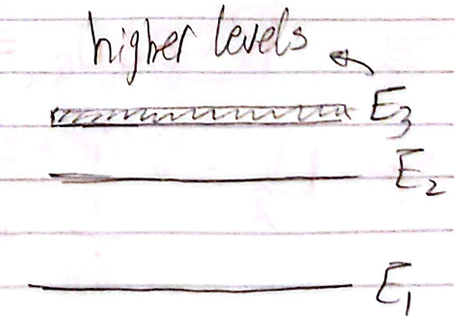
\includegraphics[scale=0.6]{1.png}
\end{minipage}
\subsection{No Input Signal or Small Signal}
\begin{align*}
    \frac{dN_2}{dt} &= R - \frac{N_{21}}{\tau_{2}}
\end{align*}
At steady state, $\frac{dN_2}{dt} = 0$, so
\begin{align*}
    N_2 &= R \tau_{21}
\end{align*}
If we use $\frac{dN_1}{dt}$, we will get the same result, so we use $N_a = N_1 + N_2$. To get population inversion:
\begin{align*}
    N_2 - N_1 &= N_2 - (N_a - N_2) = 2N_2 - N_a \\
    &= 2R \tau_{21} - N_a
\end{align*}
For population inversion, $N_2 > N_1$, so
\begin{align*}
    R > \frac{N_a}{2\tau_{21}}
\end{align*}
\subsection{Large Input Signal}
Assume steady state, so:
\begin{align*}
    \frac{dN_2}{dt} &= R - \frac{N_2}{\tau_{21}} - \sigma \phi_{\nu} N_2 + \sigma \phi_{\nu} N_1 = 0\\
    \frac{dN_1}{dt} &= - R + \frac{N_2}{\tau_{21}} + \sigma \phi_{\nu} N_2 - \sigma \phi_{\nu} N_1 = 0
\end{align*}
Using $N_1 = N_a - N_2$:
\begin{align*}
    R + \sigma \phi_{\nu} N_a &= \frac{N_2}{\tau_{21}} + 2\sigma \phi_{\nu} N_2\\
    \Rightarrow N_2 &= \frac{R + \sigma \phi_{\nu} N_a}{\frac{1}{\tau_{21}} + 2\sigma \phi_{\nu}}
\end{align*}
population inversion ($N = N_2 - N_1 = 2N_2 - N_a$):
\begin{align*}
    N &= \frac{2R + 2\sigma \phi_{\nu} N_a}{\frac{1}{\tau_{21}} + 2\sigma \phi_{\nu}} - N_a\\
    &= \frac{2R - \frac{N_a}{\tau_{21}}}{\frac{1}{\tau_{2}} + 2\sigma \phi_{\nu}} = \frac{2R \tau_{21} - N_a}{1 + 2\sigma \phi_{\nu} \tau_{21}} \\
    &= \frac{N_o}{1 + \frac{\phi}{\phi_s}}
\end{align*}
where $N_o = 2R \tau_{21} - N_a$ and $\phi_s = \frac{1}{2\sigma \tau_{21}}$. \\ \\
Since $E_1$ is the ground level, it has a large population, so to achieve population inversion, we use very large power which is inefficient. However, in 4-level lasers, both $E_1$ and $E_2$ have small number of atoms, so pumping is more efficient.

\section{2-Level Laser}
\begin{minipage}{0.5\textwidth}
    \begin{itemize}
        \item Note that in 3-level \& 4-level lasers, we pump from ground level to upper level ($E_3$), so we only consider spontaneous emission during pumping. While the input signal has energy $\Delta E = E_2 - E_1$ so we consider all light matter interaction. 
        \item In 2-level lasers, we only have 2 levels, so during pumping, we have to consider all light matter interaction (spontaneous emission + stimulated emission + absorption).
    \end{itemize}
\end{minipage}
\begin{minipage}{0.45\textwidth}
    \centering
    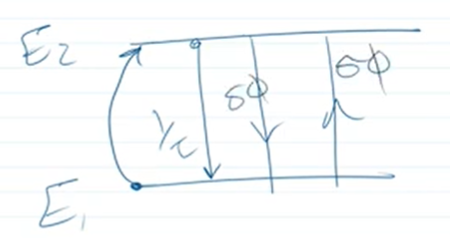
\includegraphics[scale=0.7]{2.png}
\end{minipage}
\subsection{No Input Signal or Small Signal}
We can replace the pumping rate $R$ by the absorption rate. We also have stimulated emission resulted from the light matter interaction:
\begin{align*}
    \frac{dN_2}{dt} &= - \frac{N_{21}}{\tau_{2}} - \sigma \phi_{\nu} N_2 + \sigma \phi_{\nu} (N_a - N_2) = 0 \\
    \Rightarrow N_2 &= \frac{\sigma \phi_{\nu} N_a}{\frac{1}{\tau_{2}} + 2\sigma \phi_{\nu}}
\end{align*}
Population inversion:
\begin{align*}
    N &= \frac{2\sigma \phi_{\nu} N_a}{\frac{1}{\tau_{21}} + 2\sigma \phi_{\nu}} - N_a\\
    &= \frac{-\frac{N_a}{\tau_{21}}}{\frac{1}{\tau_{2}} + 2\sigma \phi_{\nu}} < 0
\end{align*}
We can never make a laser system with 2 levels when using optical pumping. 

\section{Introduction to Semiconductor Lasers}
\subsection{Travelling Wave Amplifier (TWA)}
\begin{itemize}
    \item We pump the semiconductor with current till we reach transparency current $I_{tr}$.
    \item Trancparency current is the current at which the input power is equal to the output power.
    \item We put anti-reflection coating on the front and back of the semiconductor to prevent reflection which prevents oscillation.
    \item We can consider it as an open-loop amplifier.
    \item Small gain but high BW
\end{itemize}
\subsection{Fabry-Perot Laser (FP)}
\begin{itemize}
    \item We put a mirror on the front and back of the semiconductor.
    \item We can consider it as a positive feedback amplifier.
    \item Adjusting the mirrors (reflections) will determine wether the laser will oscillate or not (amplifier or LASER).
    \item High gain but low BW
\end{itemize}
\subsection{Erbium Doped Fiber Amplifier (EDFA)}
\begin{itemize}
    \item Regular fiber doped by Erbium, so it is a 3-level laser.
    \item The input signal is at 1550 nm, and the pump is at 980 nm.
    \item We use a directional coupler to combine the input signal and the pump.
\end{itemize}
\begin{center}
    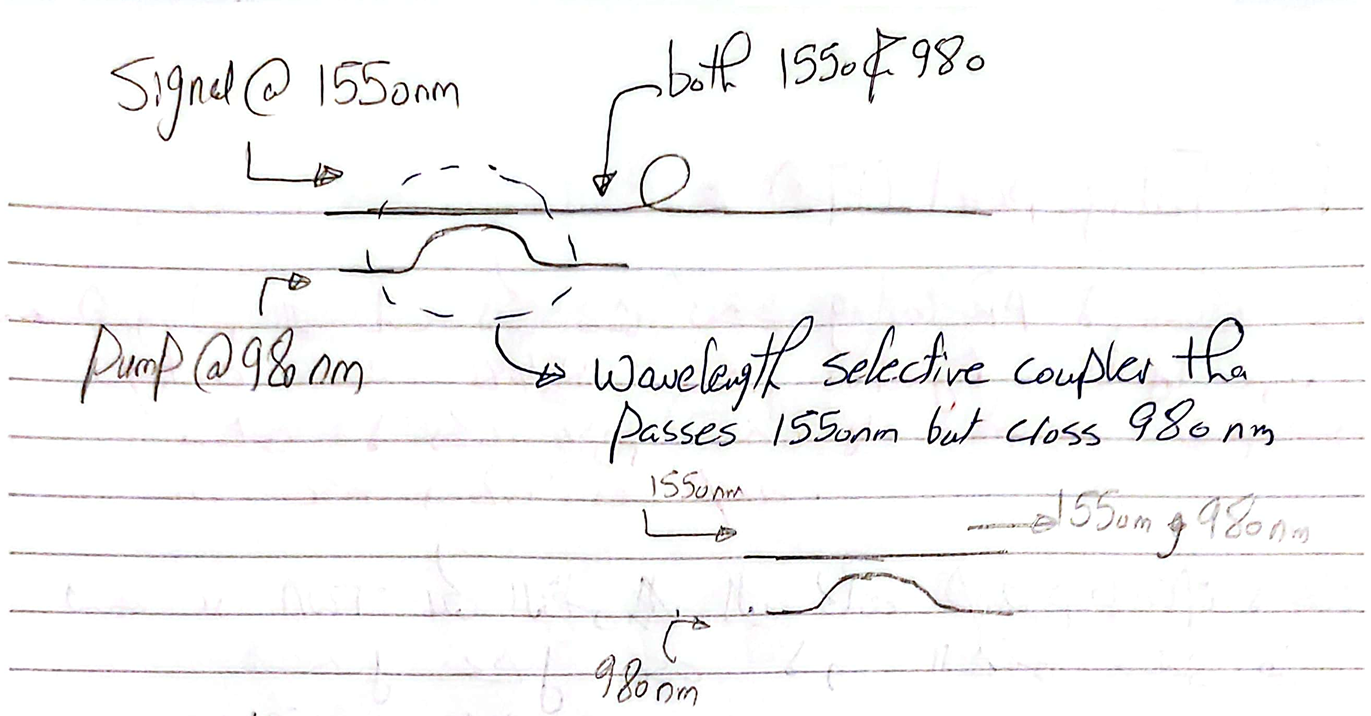
\includegraphics[scale=0.5]{3.png}
\end{center}

\section{Amplifier Noise}
\begin{itemize}
    \item Spontaneous emission is the main source of noise in amplifiers.
    \item Note that 1 atom emits 1 photon
\end{itemize}
Rate per atom:
\begin{align*}
    \frac{1}{\tau_{sp}} g_{\nu_o}(\nu) \Delta \nu
\end{align*}
Number of atoms per second per unit volume:
\begin{align*}
    \frac{1}{\tau_{sp}} g_{\nu_o}(\nu) \Delta \nu N_2 
\end{align*}
Energy of spontaneous emission per unit volume per unit time:
\begin{align*}
    \frac{1}{\tau_{sp}} g_{\nu_o}(\nu) \Delta \nu N_2 h \nu
\end{align*}
Spontaneous emission is in all directions in a Gaussian shape with a solid angle of $\frac{\lambda^2}{\text{area}}$. However, we are interested in the direction of the input signal, so:
\begin{align*}
    \text{volume} * \frac{\text{LASER solid angle}}{4\pi} = \cancel{\text{area}} \Delta z \left( \frac{\lambda^2}{4\pi \cancel{\text{area}}} \right) 
\end{align*}
Spontaneous power in the beam direction:
\begin{align*}
    dP_{ASE} &= \frac{1}{\tau_{sp}} g_{\nu_o}(\nu) \Delta \nu N_2 h \nu \Delta z \left( \frac{\lambda^2}{4\pi} \right) \\
\end{align*}
$E_x = E cos(\theta)$ and $I_x \propto E^2 cos(\theta)^2$.  For unpolarized beam, the polarization can be in any direction, so we need to take the average:
\begin{center}
    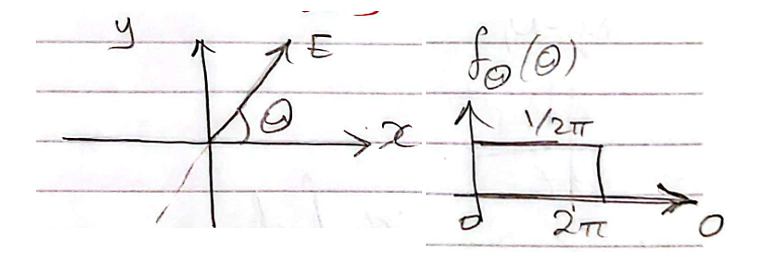
\includegraphics[scale=0.8]{4.png}
\end{center}
\begin{align*}
    <I_x> = I_o \int_{0}^{2 \pi} \frac{1}{2 \pi} \cos^2 \theta d\theta = \frac{I_o}{2}
\end{align*}
Only half the power couples the x-component, so we need to multiply by half:
\begin{align*}
    dP_{ASE} &= \frac{1}{\tau_{sp}} g_{\nu_o}(\nu) \Delta \nu N_2 h \nu \Delta z \left( \frac{\lambda^2}{4\pi} \right) \frac{1}{2} \\
\end{align*}
$\sigma = \frac{\lambda^2}{8 \pi \tau_{sp}} g_{\nu_o}(\nu)$ and  $N_2 = N_2 \frac{N_2-N_1}{N_2-N_1}$, so:
\begin{align*}
    \frac{dP_{ASE}}{dz}  &= \sigma N_2 \frac{N_2-N_1}{N_2-N_1} h \nu \Delta \nu
\end{align*}
$\gamma = \sigma (N_2 - N_1)$:
\begin{align*}
    \frac{dP_{ASE}}{dz} &= \gamma \frac{N_2}{N_2-N_1} h \nu \Delta \nu
\end{align*}
Using spontaneous emission factor $n_{sp} = \frac{N_2}{N_2-N_1}$:
\begin{align*}
    \frac{dP_{ASE}}{dz} &= \gamma n_{sp} h \nu \Delta \nu
\end{align*}
The noise spectrum is very wide, so we pass it through an optical filter of bandwidth $B_o$ so only inband noise is passed.
\begin{align*}
    \frac{dP_{ASE}}{dz} &= \gamma n_{sp} h \nu B_o
\end{align*}
\textbf{Notes:}
\begin{itemize}
    \item Net stimulated emission is proportional with $N_2-N_1$, but net spontaneous emission is proportional with $N_2$. Thus $n_{sp} = \frac{N_2}{N_2-N_1}$ is named the spontaneous emission factor.
    \item Since $N_2 > N_2 - N_1$, spontaneous emission is dominant, but since it is random, it is called noise.
    \item Spontaneous emission can happen between any 2 levels, unlike stimulated emission which only happens between $E_2$ and $E_1$ from the input signal. Therefore, spontaneous emission has a much larger bandwidth than stimulated emission.
\end{itemize}
\begin{align*}
    \frac{dP}{dz} \bigg|_{\text{total}} &= \gamma P + \gamma n_{sp} h \nu B_o
\end{align*}
Solving the differential equation assuming $\gamma = \gamma_o$ (s.s gain) and neglecting the gain saturation:
\begin{align*}
    P_{out} = G_o P_{in} + n_{sp} h \nu B_o (G_o - 1)
\end{align*}
\textbf{Notes:}
\begin{itemize}
    \item Sources of noise:
    \begin{itemize}
        \item \textbf{Relative Intensity Noise:} Fluctuations in the LASER output from the spontaneous emission.
        \begin{center}
            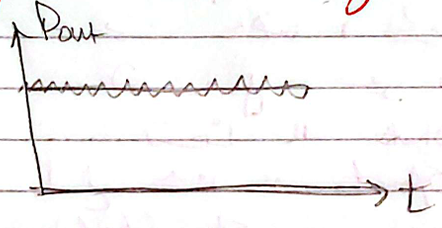
\includegraphics[scale=0.8]{5.png}
        \end{center}
        \item \textbf{Stimulated Emission Noise:} Different material interactions with the same input signal. 
    \end{itemize}
    \item Optical SNR $= \frac{P_{signal}}{P_{noise}} = \frac{G_o P_{in}}{n_{sp} h \nu B_o (G_o - 1)}$, if $G_o >> 1$, then $SNR = \frac{P_{in}}{n_{sp} h \nu B_o}$
    \item The $\nu$ used in the equations is the center of the LASER linewidth.
\end{itemize}
\begin{center}
    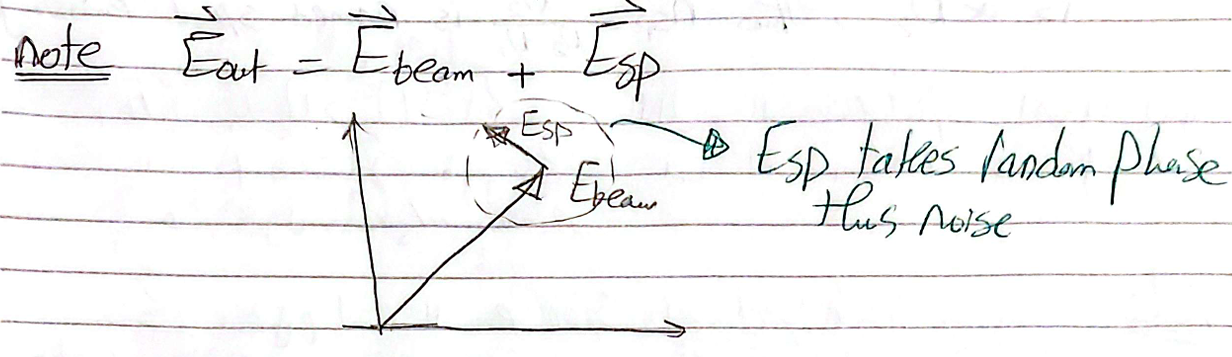
\includegraphics[scale=0.5]{6.png}
\end{center}

\section{LASER}
A LASER is an oscillator, so we need to achieve the positive feedback conditions:
\begin{itemize}
    \item Starting Noise (spontaneous emission noise).
    \item Feedback (mirrors).
    \item $A \beta > 1$ which reaches $A \beta = 1$ due to non-linearities (A is from material amplification, and $\beta$ is from the refelectance of the mirrors).
\end{itemize}
\subsection{Types of Mirrors}
\begin{minipage}{0.5\textwidth}
    \begin{itemize}
        \item \textbf{Simple Discontinuity:}
            \begin{itemize}
                \item $\Gamma = \frac{n-1}{n+1}$ (real)
                \item The normal case in semiconductor lasers.
            \end{itemize}
        \item \textbf{Dielectric Slab:}
            \begin{itemize}
                \item $\Gamma$ can be complex dependeing on time.
                \item The normal case in gas.
            \end{itemize}
    \end{itemize}
\end{minipage}
\begin{minipage}{0.45\textwidth}
    \centering
    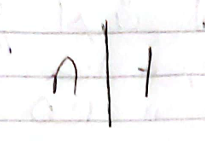
\includegraphics[scale=0.6]{9.png} \\
    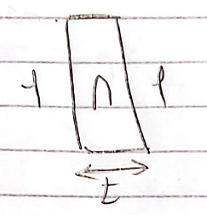
\includegraphics[scale=0.6]{10.png}
\end{minipage}


\subsection{Phase Condition}
\begin{center}
    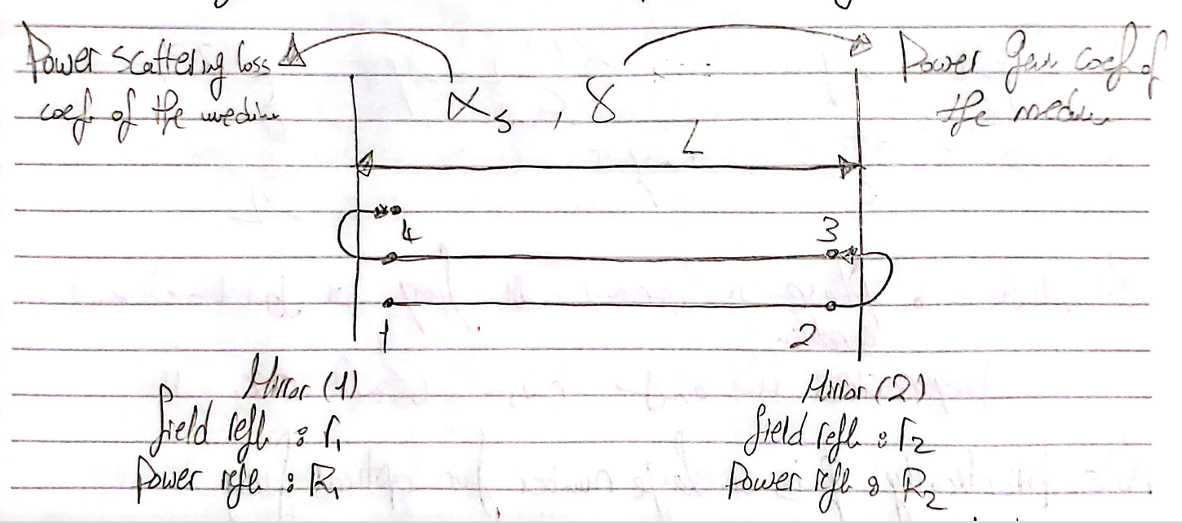
\includegraphics[scale=0.65]{7.png}
\end{center}
Assuming constant gain ($\gamma$):
\begin{align*}
    E_1 \\
    E_2 &= E_1 e^{-j \beta L} e^{-\frac{\alpha_s}{2} L} e^{\frac{\gamma}{2} L} \\
    E_3 &= r_2 E_1 e^{-j \beta L} e^{-\frac{\alpha_s}{2} L} e^{\frac{\gamma}{2} L} \\
    E_4 &= r_2 E_1 e^{-2j \beta L} e^{-\alpha_s L} e^{\gamma L} \\
    E_5 &= r_1 r_2 E_1 e^{-2j \beta L} e^{-\alpha_s L} e^{\gamma L} \\
\end{align*}
For oscillation, $E_1$ should add with $E_5$:
\begin{align*}
    2 \beta L &= 2 q \pi \Rightarrow 2 \frac{\omega}{c} L = 2 q \pi \\
    2 \frac{2 \pi \nu}{c} L &= 2 q \pi \Rightarrow \nu = \frac{qc}{2L}
\end{align*}
where $q$ is an integer. Practically $q$ is a large number $\approx 10^2$. 

\subsection{Gain Condition}
\begin{align*}
    r_1 r_2 e^{-\alpha_s L} e^{\gamma L} > 1
\end{align*}
So:
\begin{align*}
    e^{\gamma L} &> \frac{e^{\alpha_s L}}{r_1 r_2} \Rightarrow \gamma L > \alpha_s L + \ln(\frac{1}{r_1 r_2}) \\
    \gamma &> \alpha_s + \frac{1}{L} \ln \left( \frac{1}{r_1 r_2} \right)
\end{align*}
$r_1 = \sqrt{R_1}$ and $r_2 = \sqrt{R_2}$, so:
\begin{align*}
    \gamma &> \alpha_s + \frac{1}{2L} \ln \left( \frac{1}{R_1 R_2} \right)
\end{align*}
where:
\begin{itemize}
    \item $\alpha_s$ is the scattering loss and other losses (apart from absorption as it is included in the gain $\gamma$). 
    \item $\frac{1}{2L} \ln \left( \frac{1}{R_1 R_2} \right)$ is the mirror loss (if $R_1=R_2=1$ this term is 0).
    \item $\alpha_s + \frac{1}{2L} \ln \left( \frac{1}{R_1 R_2} \right)$ is called the resonator loss ($\alpha_r$). For amplification, $\gamma > \alpha_r$.
    \item We assumed that both $r_1$ and $r_2$ are real so they only affect the gain condition, but the general case is that they are complex, so they affect the phase condition as well.
\end{itemize}

\section{Conclusion}
For oscillation, we must satisfy both conditions:
\begin{itemize}
    \item Phase condition: $\nu = \frac{qc}{2L}$
    \item Gain condition: $\gamma > \alpha_r$
\end{itemize}
Gain peak is lower than $\alpha_r \Rightarrow$ No oscillation. 
\begin{center}
    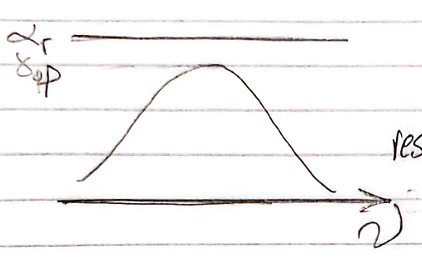
\includegraphics[scale=0.8]{11.png}
\end{center}
Oscillation only happens at $\nu_q$, $\nu_{q+1}$, $\nu_{q-1}$:
\begin{center}
    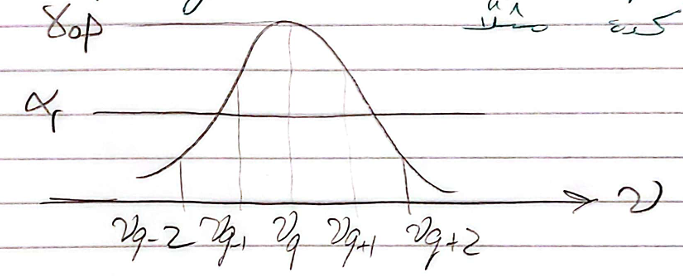
\includegraphics[scale=0.8]{12.png}
\end{center}
As light intensity increases, the gain decreases, so the gain curve moves down, so some modes will stop oscillating ($\gamma < \alpha_r$) even if they satisfy the phase condition.


\end{document}